% Sketch output, version 0.3 (build 2d, Wed Apr 20 23:38:45 2011)
% Output language: PGF/TikZ,LaTeX
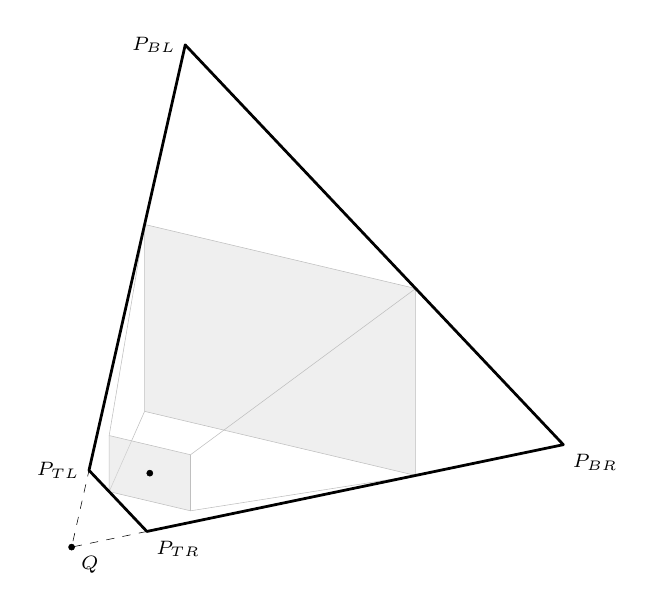
\begin{tikzpicture}[line join=round,line width=0.2pt,>=latex]
\filldraw[color=lightgray,fill=lightgray!50,fill opacity=0.5](4.085,3.016)--(.643,3.83)--(.643,1.456)--(4.085,.642)--cycle;
\draw[color=lightgray](.193,.437)--(.643,1.456);
\draw[color=lightgray](.193,1.149)--(.643,3.83);
\draw[color=lightgray](1.226,.193)--(4.085,.642);
\draw[color=lightgray](1.226,.905)--(4.085,3.016);
\filldraw[color=lightgray,fill=lightgray!50,fill opacity=0.5](1.226,.905)--(.193,1.149)--(.193,.437)--(1.226,.193)--cycle;
\draw[dashed](.672,-.069)--(-.284,-.268)--(-.063,.707);
\filldraw[](.709,.671) circle (1.1pt);
\filldraw[](-.284,-.268) circle (1.1pt);
\filldraw[fill=none,line width=1pt](-.063,.707)--(1.159,6.11)--(5.961,1.033)--(.672,-.069)--cycle;

    \coordinate [label=-45:\scriptsize$Q$] (Q) at (-.284,-.268);
    \coordinate [label=180:\scriptsize$P_{TL}$] (Ptl) at (-.063,.707);
    \coordinate [label=180:\scriptsize$P_{BL}$] (Pbl) at (1.159,6.11);
    \coordinate [label=-60:\scriptsize$P_{TR}$] (Ptr) at (.672,-.069);
    \coordinate [label=-60:\scriptsize$P_{BR}$] (Pbr) at (5.961,1.033);
  \end{tikzpicture}% End sketch output
